\documentclass[aspectratio=43]{beamer}
\beamertemplatenavigationsymbolsempty
\usecolortheme{beaver}
\setbeamertemplate{blocks}[rounded=true, shadow=true]
\setbeamertemplate{footline}[page number]
\usefonttheme[onlymath]{serif}

\usepackage[utf8]{inputenc}
\usepackage[english,russian]{babel}
\usepackage{amssymb,amsfonts,amsmath,mathtext}
\usepackage{subfig}
\usepackage{array}
\usepackage{bm}
\usepackage{multicol}
\usepackage{hyperref}
\usepackage{hhline}
\usepackage{subcaption}
\usepackage{accents}
\usepackage{booktabs}
\usepackage{mathtools}
\usepackage{graphicx}
\usepackage{adjustbox}
\usepackage{ragged2e}
\setbeamertemplate{theorems}[numbered]
\setbeamertemplate{caption}[numbered]

\input{newcommands}

\title[\hbox to 56mm{Декодирование визуальной информации из сигналов мозга}]{Декодирование визуальной информации из сигналов мозга на основе пространственно- временных характеристик}
\author[Д.\,Д.~Дорин]{Даниил Дмитриевич Дорин\\
\small Научный руководитель: к.ф.-м.н. А.\,В.~Грабовой}

\institute{
    Кафедра интеллектуальных систем ФПМИ МФТИ\\
    Специализация: Интеллектуальный анализ данных\\
    Направление: 09.04.01 Информатика и вычислительная техника
}
\date{Москва --- 2026}

\begin{document}

\begin{frame}
\thispagestyle{empty}
\maketitle
\end{frame}
%----------------------------------------------------------------------------------------------------------
\begin{frame}{Декодирование визуальных стимулов из сигналов мозга}
\begin{block}{Цель исследования}
\justifying
Разработать метод декодирования визуальных стимулов по мультимодальным сигналам мозга на основе пространственно-временных характеристик.
\end{block}
\begin{block}{Задача}
\justifying
Предложить метод декодирования временных рядов фМРТ в условиях ограниченного объема выборки. Показать повышение качества при использовании нескольких модальностей.
\end{block}
\begin{block}{Методы решения}
\justifying
\begin{enumerate}
\justifying
    \item Учесть время через анализ гемодинамического лага.
    \item Описать пространственную структуру фМРТ с помощью масок активности и римановой геометрии.
    \item Добавить модальность ЭЭГ для демонстрации дополняющих характеристик.
\end{enumerate}
\end{block}
\end{frame}
%----------------------------------------------------------------------------------------------------------
\begin{frame}{Постановка задачи}
\justifying
Пусть $\mathcal{X}_{(m)}$ обозначает пространство наблюдений модальности $m$, где $m = 1, \ldots, M$. 
Тогда совместное пространство нейробиологических данных
\[
\mathcal{X} = \mathcal{X}_{(1)} \times \ldots \times \mathcal{X}_{(M)}.
\]
Визуальный стимул или его характеристика $\mathbf{y} \in \mathcal{Y}$.
Требуется построить отображение декодирования
\[
\mathbf{g}: \mathcal{X} \rightarrow \mathcal{Y}.
\]

\begin{block}{Частные случаи}
    Классификация временных рядов фМРТ
        \[
        \mathbf{g}: \mathcal{X}_{f} \rightarrow \{1,\ldots,C\}.
        \]
    Реконструкция изображений по совместным фМРТ--ЭЭГ
        \[
        \mathbf{g}: \mathcal{X}_{f} \times \mathcal{X}_{e} \rightarrow \mathcal{Y}.
        \]
\end{block}
\end{frame}
%----------------------------------------------------------------------------------------------------------
\begin{frame}{Линейная модель прогнозирования фМРТ-отклика}
\justifying
Сигнал фМРТ возникает с \textbf{гемодинамическим лагом} $\Delta t$ относительно стимула. Для согласования их временных шкал решается обратная к декодированию задача.

\begin{block}{Авторегрессионная марковская модель}
\[
\mathbf{g}(\mathbf{y}_{k_{\ell} - \nu \Delta t}) = \mathbf{X}_{\ell} - \mathbf{X}_{\ell-1}, \quad k_{\ell} = \dfrac{\ell \cdot \nu}{\mu},
\]
где $\mu$, $\nu$~-- частоты дискретизации фМРТ и видеоряда, а лаг~$\Delta t$ сдвигает стимул в прошлое.
\end{block}

Параметры линейной модели~$\mathbf{W}$ оцениваются на обучающей выборке, лаг~$\Delta t$~-- по ошибке восстановления на тестовой:
\[
\widehat{\mathbf{W}}(\Delta t) = \argmin_{\mathbf{W}} \!\!\sum_{\ell \in \text{train}} \!\! \big\| \mathbf{g}(\mathbf{y}_{k_{\ell} - \nu \Delta t}) - (\mathbf{X}_{\ell} - \mathbf{X}_{\ell-1}) \big\|_2^2 + \lambda \|\mathbf{W}\|_F^2,
\]
\end{frame}
%----------------------------------------------------------------------------------------------------------
\begin{frame}{Оценка гемодинамического лага}
\justifying
Модель обучается индивидуально для испытуемого при каждом~$\Delta t$; MSE усредняется по вокселям и объектам тестовой выборки.

\begin{figure}
    \centering
    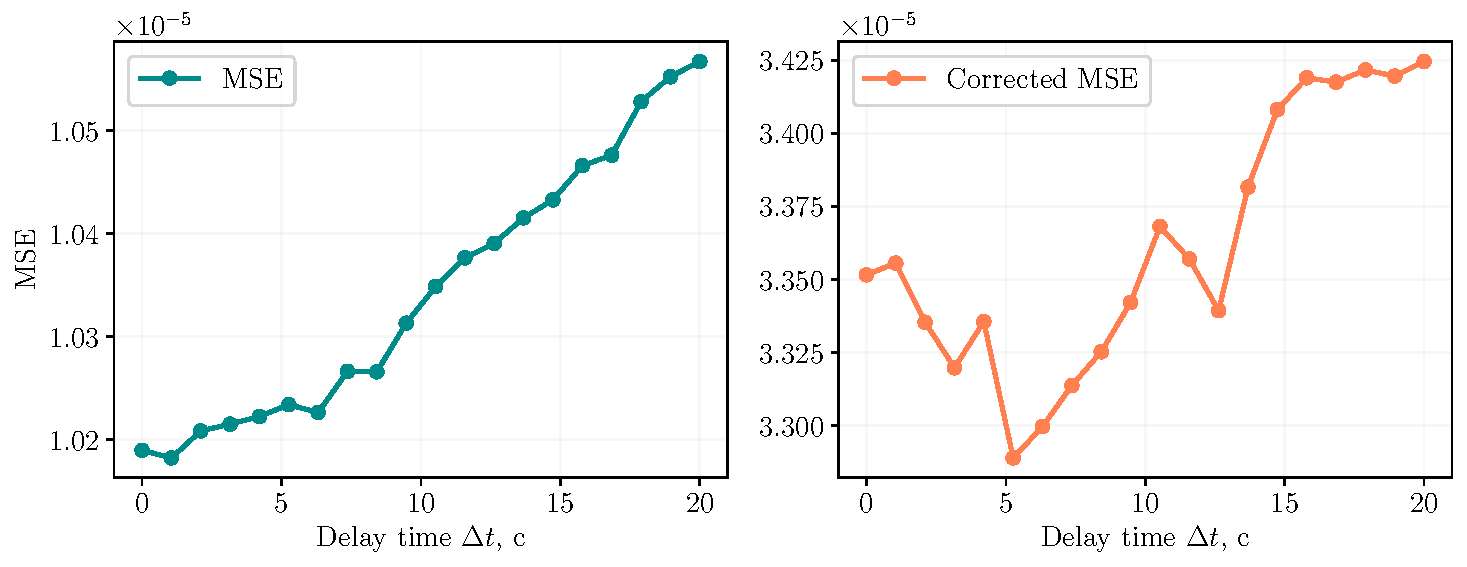
\includegraphics[width=1.\linewidth]{figs/mse_dt.pdf}
\end{figure}

\vspace{-0.3em}
Зависимость MSE от $\Delta t$ имеет минимум; на локализованной зрительной коре он отчетливо выражен. Полученное значение согласуется с нейрофизиологическими оценками.
\end{frame}
%----------------------------------------------------------------------------------------------------------
\begin{frame}{Схема метода классификации фМРТ}
\justifying
\hspace{-0.12cm}
\begin{figure}
	\centering
	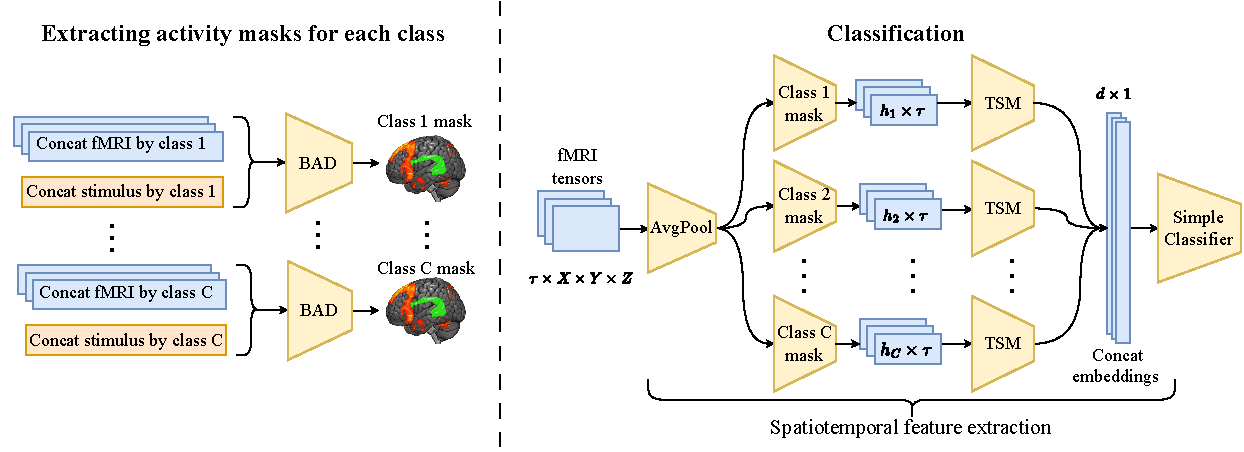
\includegraphics[width=1.\linewidth]{figs/Figure_2.pdf}
\end{figure}
\vspace{-4mm}
Метод строится из двух этапов~-- извлечение масок активности головного мозга для каждой категории стимула и классификация с учетом полученных масок.
\end{frame}
%----------------------------------------------------------------------------------------------------------
\begin{frame}{Метод классификации временных рядов фМРТ}
\small
Отображение $\mathbf{g}: \mathcal{X}_{f} \rightarrow \{1,\ldots, C\}$~-- суперпозиция $\mathbf{g} = \bm{\varphi} \circ \bm{\psi} \circ \mathcal{A}$
\begin{align*}
    & \mathcal{A}: \mathcal{X}_{f} \to \mathbb{R}^{\tau \times X/k_s \times Y/k_s \times Z/k_s}
    \text{~-- Average Pooling}        \\
    & \bm{\psi}: \mathbb{R}^{\tau \times X/k_s \times Y/k_s \times Z/k_s} \to \mathbb{R}^d
    \text{~-- векторизатор}        \\
    & \bm{\varphi}: \mathbb{R}^d \to \{1,\ldots, C\}
    \text{~-- классификатор (Logistic Regression)}
\end{align*}
Отображение $\bm{\psi}$~-- конкатенация $\bm{\psi} = \bm{\psi}_1 \oplus \ldots \oplus \bm{\psi}_C$
\begin{align*}
    & \bm{\psi}_k: \mathbb{R}^{\tau \times X/k_s \times Y/k_s \times Z/k_s} \rightarrow \mathbb{R}^{d_k},
    \quad \bm{\psi}_k = \bm{\pi}_k \circ \bm{f}_k,
    \quad d = \sum_{k=1}^C \underbrace{\dfrac{h_k(h_k+1)}{2}}_{\textstyle d_k}, \\
    & \bm{f}_k: \mathbb{R}^{\tau \times X/k_s \times Y/k_s \times Z/k_s} \rightarrow \mathbb{R}^{h_k \times \tau}~\text{применяет маску активности}~\mathcal{M}^k, \\
    & \bm{\pi}_k: \mathbb{R}^{h_k \times \tau} \rightarrow \mathbb{R}^{d_k}~\text{проекция на риманово касательное пространство,}
\end{align*}
где $h_k$~-- число ненулевых элементов в $\mathcal{M}^k$~-- сжатая маска активности класса $k$.
\end{frame}
%----------------------------------------------------------------------------------------------------------
\begin{frame}{Проекция на риманово касательное пространство}
\justifying
Ковариационная матрица \(\mathbf{R}_j\) проецируется на касательное пространство \(T_\mathbf{R}\) в точке \(\mathbf{R}\) с использованием отображения \(\operatorname{Log}_{\mathbf{R}}(\mathbf{R}_j)\). Полученная проекция \(\mathbf{P}_j\) затем отображается обратно на риманово многообразие \(\mathcal{R}\) с использованием \(\operatorname{Exp}_{\mathbf{R}}(\mathbf{P}_j)\).
\begin{figure}
    \centering
    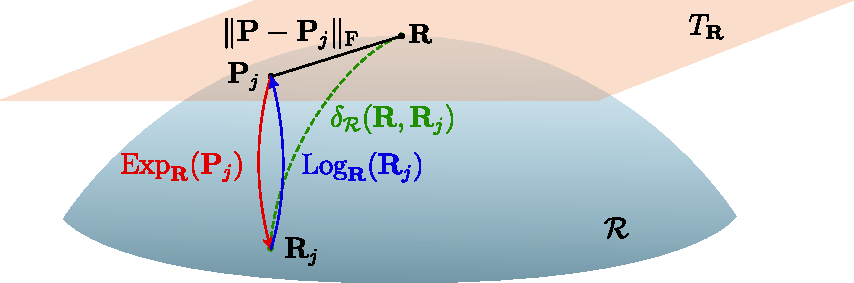
\includegraphics[width=0.7\linewidth]{figs/Figure_3.pdf}
    \label{fig:riman}
\end{figure}
\begin{itemize}
    \item \(\delta_{\mathcal{R}}(\mathbf{R},~\mathbf{R}_j)\) — геодезическое расстояние между \(\mathbf{R}\) и \(\mathbf{R}_j\)
    \item $\operatorname{Log}_{\mathbf{R}}(\mathbf{R}_j) = \mathbf{R}^{\frac{1}{2}} \log\left(\mathbf{R}^{-\frac{1}{2}}\mathbf{R}_j\mathbf{R}^{-\frac{1}{2}}\right) \mathbf{R}^{\frac{1}{2}} \in T_\mathbf{R}$
    \item $\operatorname{Exp}_{\mathbf{R}}(\mathbf{P}_j) = \mathbf{R}^{\frac{1}{2}} \exp\left(\mathbf{R}^{-\frac{1}{2}}\mathbf{P}_j\mathbf{R}^{-\frac{1}{2}}\right) \mathbf{R}^{\frac{1}{2}} \in \mathcal{R}$
\end{itemize}

\end{frame}
%----------------------------------------------------------------------------------------------------------
\begin{frame}{Анализ алгоритма декодирования активности мозга}
\justifying
\begin{itemize}
    \item Рассматривается датасет Haxby et al. Взяты данные фМРТ 1-го испытуемого.
    \item Частота снимков $\mu=2.5~\text{с}^{-1}$, число областей $h=10$, размер ядра $k_s=4$.
\end{itemize}
\vspace{-0.25cm}
\begin{figure}[h!]
	\centering
	\subfloat[\centeringАлгоритм]{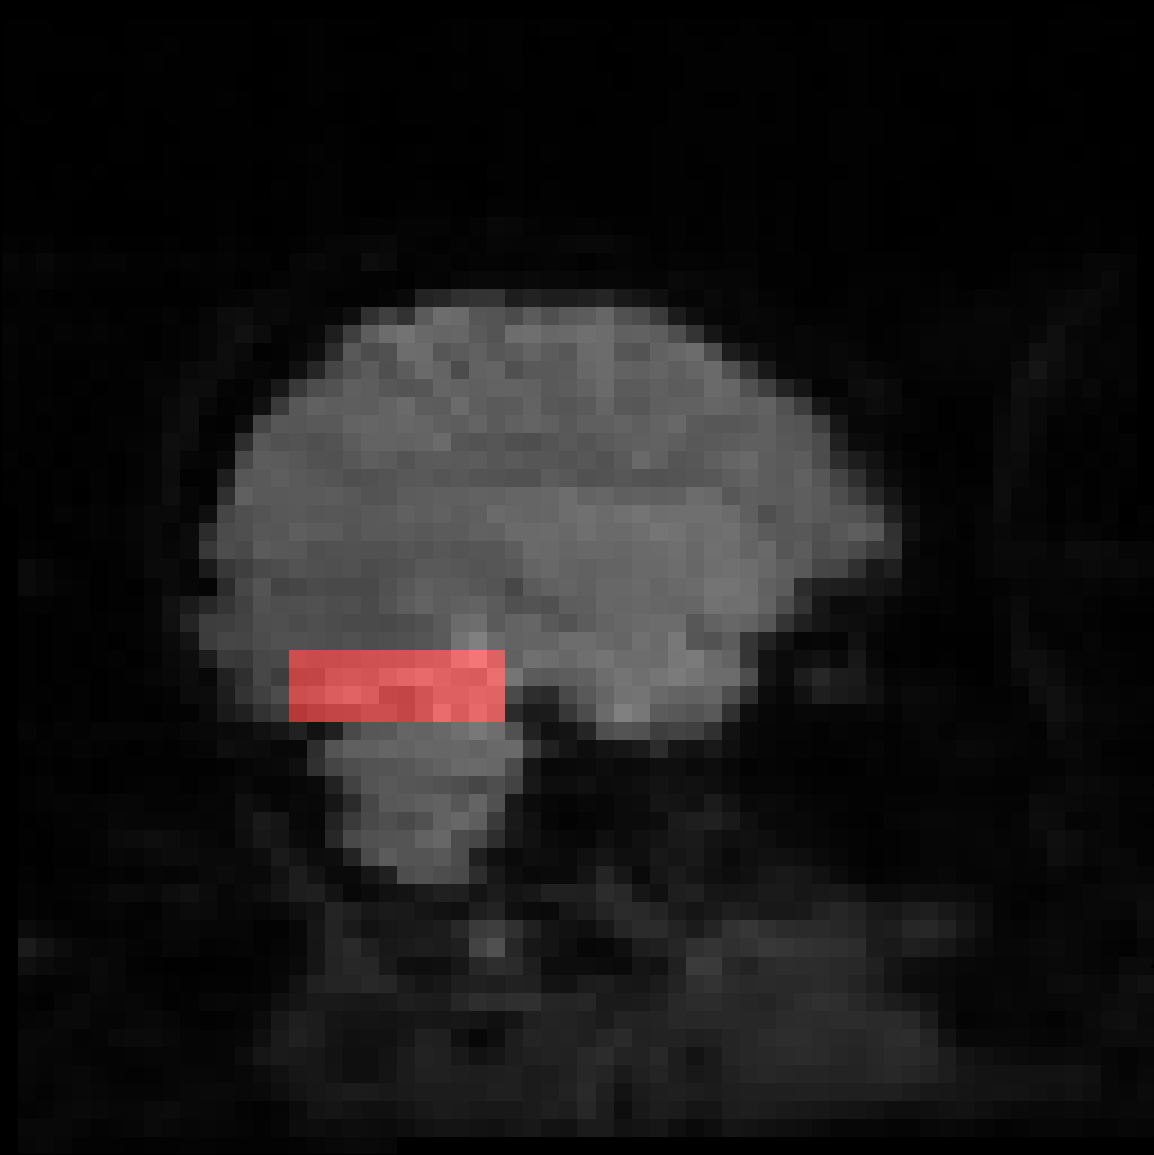
\includegraphics[width=0.26\textwidth]{figs/Figure_5.png}}\hfill
	\subfloat[\centeringСтатистически значимые области]{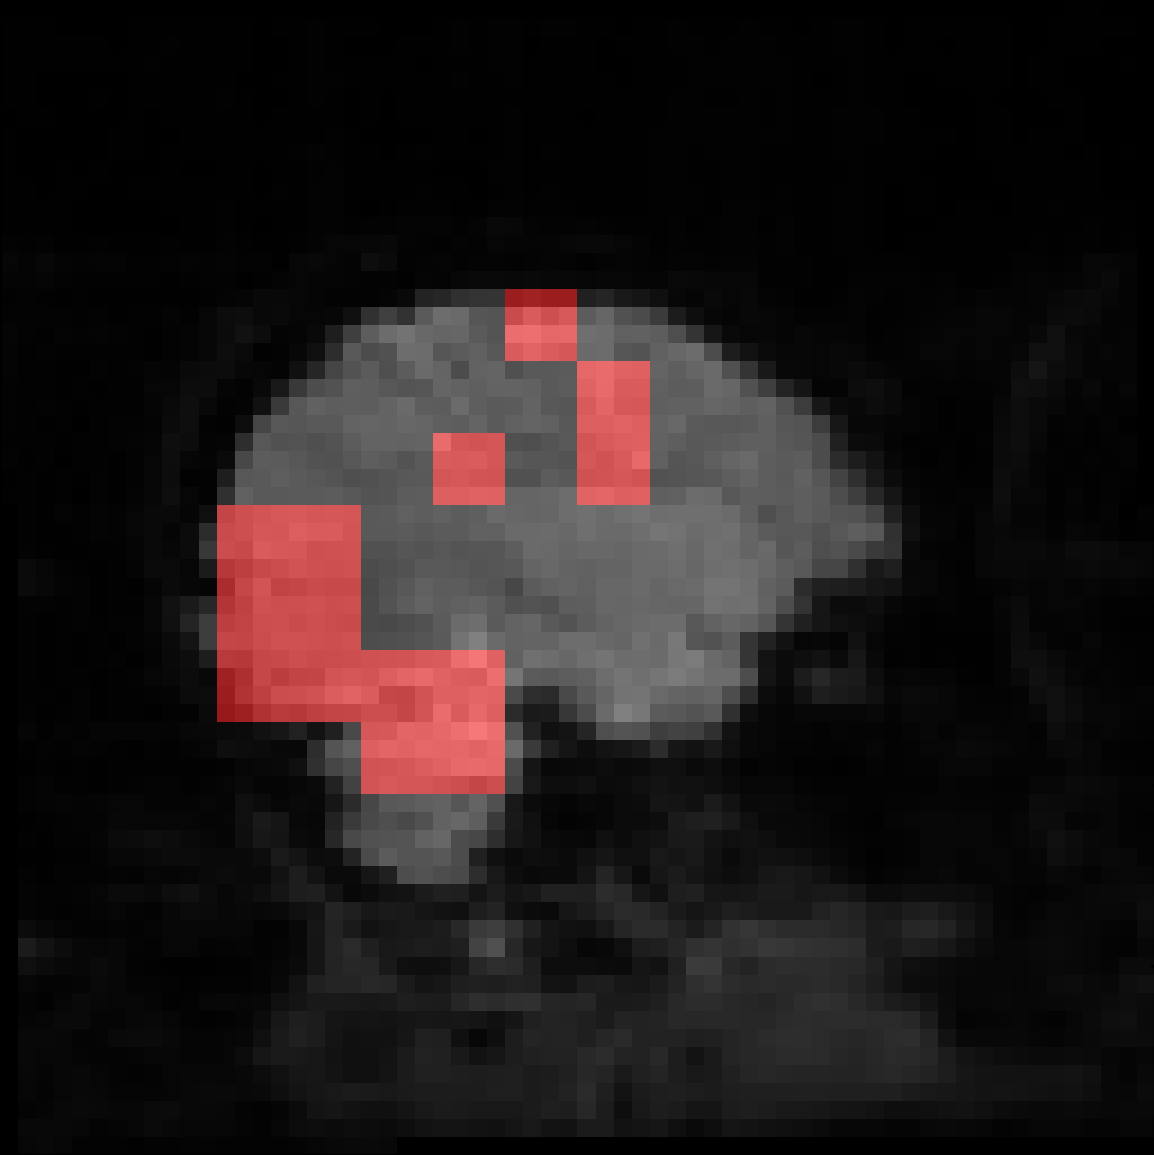
\includegraphics[width=0.26\textwidth]{figs/Figure_6.png}}\hfill
	\subfloat[\centeringРазметка нейробиологов]{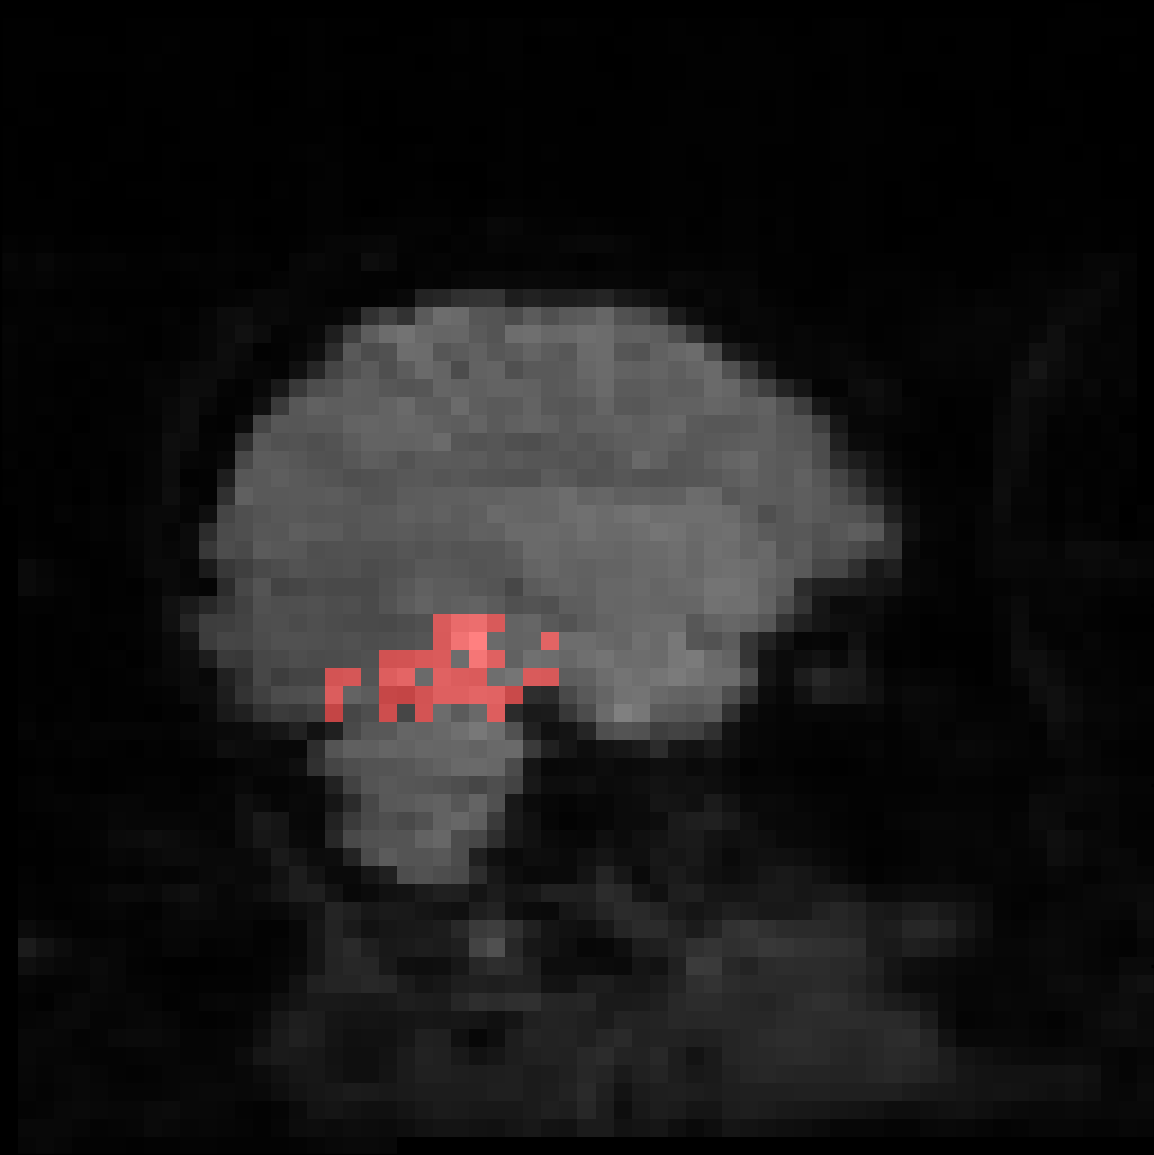
\includegraphics[width=0.26\textwidth]{figs/Figure_7.png}}
\end{figure}
Полученные области покрывают разметку нейробиологов. Корреляция взвешенных областей со стимулом стат. значима.
\end{frame}
%----------------------------------------------------------------------------------------------------------
\begin{frame}{Анализ компонент и сравнение с нейросетями}
\justifying
Рассматривается датасет Haxby et al., состоящий из данных 6 испытуемых, объём $N=96$, число классов $C=8$. Тестовая выборка~-- 20\%. Метрики усреднены по 6 выборкам. Статистическая значимость обозначена *$p<.05$, **$p<.005$.

\medskip
\textbf{Анализ исключением компонент.} Рассматриваются 3 упрощённые модели. Указаны $95\%$ доверительные интервалы.
\par\nobreak\vspace{1.5mm}
\noindent\resizebox{\textwidth}{!}{%
\begin{tabular}{l ccc ccc}
    \toprule
    Method & Accuracy & Macro F1-Score & Micro F1-Score & Accuracy CI & Macro F1 CI & Micro F1 CI \\
    \midrule
    Ours, w/o TSM & 0.24 $\pm$ 0.11* & 0.22 $\pm$ 0.11* & 0.24 $\pm$ 0.11* & [0.11, 0.37] & [0.09, 0.36] & [0.10, 0.37] \\
    Ours, w/o Class Masks & 0.25 $\pm$ 0.13* & 0.23 $\pm$ 0.13* & 0.25 $\pm$ 0.13* & [0.09, 0.41] & [0.07, 0.39] & [0.09, 0.41] \\
    Ours, Original Mask & 0.10 $\pm$ 0.05** & 0.09 $\pm$ 0.04** & 0.10 $\pm$ 0.05** & [0.04, 0.16] & [0.03, 0.14] & [0.04, 0.16] \\
    Ours & \textbf{0.61 $\pm$ 0.04} & \textbf{0.56 $\pm$ 0.03} & \textbf{0.61 $\pm$ 0.04} & [0.56, 0.66] & [0.52, 0.60] & [0.56, 0.66] \\
    \bottomrule
\end{tabular}}

\bigskip
\textbf{Сравнение с нейросетевыми решениями.}
\par\nobreak\vspace{1.5mm}
\noindent\resizebox{\textwidth}{!}{%
\begin{tabular}{l ccc ccc}
    \toprule
    Model & Accuracy & Macro F1-Score & Micro F1-Score & Accuracy CI & Macro F1 CI & Micro F1 CI \\
    \midrule
    Original Mask \& LSTM & 0.12 $\pm$ 0.02** & 0.03 $\pm$ 0.01** & 0.12 $\pm$ 0.02** & [0.09, 0.14] & [0.02, 0.04] & [0.09, 0.14] \\
    Original Mask \& Attention & 0.14 $\pm$ 0.04** & 0.04 $\pm$ 0.03** & 0.14 $\pm$ 0.04** & [0.11, 0.18] & [0.02, 0.07] & [0.11, 0.18] \\
    Ours, Logistic Regression $\bm{\varphi}$ & \textbf{0.61 $\pm$ 0.04} & \textbf{0.56 $\pm$ 0.03} & \textbf{0.61 $\pm$ 0.04} & [0.56, 0.66] & [0.52, 0.60] & [0.56, 0.66] \\
    \bottomrule
\end{tabular}}
\end{frame}
%----------------------------------------------------------------------------------------------------------
\begin{frame}{Реконструкция стимула по данным  фМРТ--ЭЭГ}
\justifying
\vspace{-1.5mm}
Задан датасет триплетов (фМРТ, ЭЭГ, изображение):
\[
\mathfrak{D}=\{(\mathbf{F}_i,\mathbf{E}_i,\mathbf{I}_i)\mid i=1,\ldots,N\},\quad (\mathbf{F}_i,\mathbf{E}_i)\in\mathcal{X}_{f}\times\mathcal{X}_{e},\quad \mathbf{I}_i\in\mathcal{Y}.
\]
Требуется построить отображение $\mathbf{g}:\mathcal{X}_{f}\times\mathcal{X}_{e}\rightarrow\mathcal{Y}.$
\begin{block}{Решение в два этапа:}
    \justifying
    Контрастивное обучение объединенных представлений фМРТ--ЭЭГ и реконструкция стимулов с помощью двустадийной диффузионной генерации.
\end{block}
\vspace{-1mm}
\begin{figure}
    \centering
    
\includegraphics[width=0.75\linewidth]{figs/scheme.pdf}
\end{figure}
\end{frame}

\begin{frame}{Контрастивное обучение представлений фМРТ--ЭЭГ}
\justifying
\vspace{-1mm}
Используется косинусное расстояние между эмбеддингами для вычисления матрицы логитов \( \mathbf{L} \):
    \begin{equation*}
        \mathbf{Z}_I^n = \frac{\mathbf{Z}_I}{\|\mathbf{Z}_I\|}, \quad \mathbf{Z}_c^n = \frac{\mathbf{Z}_c}{\|\mathbf{Z}_c\|}, \quad \mathbf{L} = \mathbf{Z}_I^n \left(\mathbf{Z}_c^n\right)^{\T} \cdot e^{\tau}
\end{equation*}
где $\tau$~--- обучаемый параметр температуры.
%----------------------------------------------------------------------------------------------------------
\begin{block}{Симметричная контрастивная функция потерь}
\begin{equation*}
\mathcal{L} = -\frac{1}{2B} \sum_{b=0}^{B-1} \log \left( \frac{\exp(\mathbf{L}_{bb})}{\sum_{j=0}^{B-1} \exp(\mathbf{L}_{bj})} \right) + \log \left( \frac{\exp(\mathbf{L}_{bb})}{\sum_{i=0}^{B-1} \exp(\mathbf{L}_{ib})} \right) 
\end{equation*}
Здесь \( \mathbf{L}_{ij} \)~-- это элемент матрицы логитов \( \mathbf{L} \) на позиции \( (i,~j) \). 

\begin{figure}
    \centering
    \includegraphics[width=0.5\linewidth]{figs/triplet-loss.png}
\end{figure}
\end{block}
\end{frame}
%----------------------------------------------------------------------------------------------------------
\begin{frame}{Оценка мультимодальной модели}
\justifying
Для оценки качества модели используется CLIP-Score, так как мы сопоставляем объединенные эмбеддинги с эмбеддингами изображений CLIP:
    \[
        \text{CLIP-Score}(\mathbf{z}_c, \mathbf{z}_I) = \frac{\langle \mathbf{z}_c, \mathbf{z}_I \rangle}{\| \mathbf{z}_c \| \| \mathbf{z}_I \|}.
    \]
    Этот показатель рассчитывается для каждого триплета в тестовом наборе данных.
\begin{table}
    \centering
    \resizebox{0.94\textwidth}{!}{
    \begin{tabular}{lccc}
        \toprule
        Модель & \texttt{monkey1} & \texttt{monkey2} & \texttt{monkey5} \\
        \midrule
        ЭЭГ & $0.231_{\pm 0.004}$ & $0.262_{\pm 0.004}$ & $0.224_{\pm 0.005}$ \\
        фМРТ & $0.254_{\pm 0.004}$ & $0.270_{\pm 0.003}$ & $0.242_{\pm 0.003}$ \\
        фМРТ--ЭЭГ & $0.310_{\pm 0.003}$ & $0.312_{\pm 0.004}$ & $0.284_{\pm 0.003}$ \\
        ЭЭГ \& Diffusion Prior & $0.542_{\pm 0.005}$ & $0.557_{\pm 0.003}$ & $0.538_{\pm 0.003}$ \\
        фМРТ \& Diffusion Prior & $0.564_{\pm 0.005}$ & $0.571_{\pm 0.004}$ & $0.551_{\pm 0.005}$ \\
        фМРТ--ЭЭГ \& Diffusion Prior & $\mathbf{0.668}_{\pm 0.003}$ & $\mathbf{0.647}_{\pm 0.005}$ & $\mathbf{0.644}_{\pm 0.003}$ \\
        \bottomrule
    \end{tabular}
    }
\end{table}
\vspace{-0.2em}
Мультимодальная модель фМРТ--ЭЭГ превосходит одномодальные аналоги
\end{frame}
%----------------------------------------------------------------------------------------------------------
\begin{frame}{Примеры реконструкции изображений}
\justifying
Реконструкция по одновременным данным фМРТ-ЭЭГ. 
\begin{figure}
    \centering
    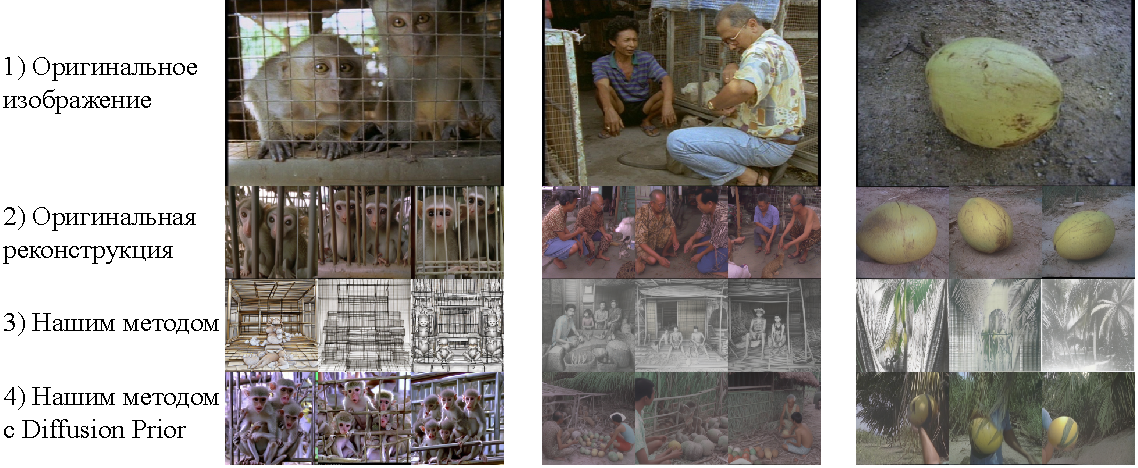
\includegraphics[width=0.9\linewidth]{figs/examples.pdf}
\end{figure}
Модель успешно реконструирует семантику визуальных стимулов, просматриваемых испытуемым.
\end{frame}

\begin{frame}{Выносится на защиту}
\footnotesize
\begin{enumerate}
\justifying
    \item Построен метод восстановления показаний фМРТ по видеоряду, просматриваемому человеком. Обоснован учет гемодинамического лага.
    \item Разработан метод классификации временных рядов фМРТ в услових ограниченного объема выборки. Предложен алгоритм декодирования активности мозга.
    \item Предложен метод реконструкции изображений по совместным сигналам фМРТ--ЭЭГ. Интеграция мультимодальности фМРТ--ЭЭГ улучшает декодирование за счет пространственно-временной комплементарности.
\end{enumerate}
\footnotesize
\begin{block}{\small Публикации в журналах ВАК по теме доклада}
\begin{enumerate}
\justifying
    \item \textit{\textbf{Dorin D}., Kiselev N. et al.} Forecasting fMRI Images From Video Sequences: Linear Model Analysis // Health Information Science and Systems.~-- 2024.
    \item \textit{\textbf{Dorin D.} et al.} Enhancing fMRI Data Decoding with Spatiotemporal Characteristics in Limited Dataset // Doklady Mathematics.~-- 2025.
    \item \textit{\textbf{Dorin D.} et al.} Decoding Visual Information from Neural Signals: Image Reconstruction Based on Joint fMRI and EEG Analysis // Informatika i ee Primeneniya.~-- 2026.
\end{enumerate}
\end{block}
\end{frame}
%---------------------------------------------------------------------------------------------------------
\end{document}